\section{无延迟策略的模仿学习}

核心理念如\Cref{fig:imitation_delay_explanation}所示，即模仿无延迟专家在当前未观测状态上会执行的策略。
由于当前状态未知，只能根据增广状态计算其信念。
因此，延迟策略学习在信念分布下复制无延迟策略的动作。
使用 \textsc{DAgger}~\cite{ross2011reduction} 作为模仿学习算法，因其能够考虑专家与学习器策略之间的分布偏移，如\Cref{subsec:imitation_learning}所述。
这是一项重要性质，因为延迟加剧了状态分布的偏移。
该偏移将在\Cref{subsec:analysis_ismmdp}中详细讨论。

\begin{figure}[t]
    \centering
    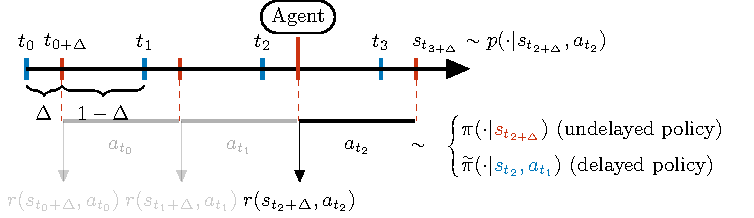
\includegraphics[labelimitation=dualitytrajectory]{img/thesis_plots_imitation.pdf}
    \caption{无延迟策略 $\pi$（专家）被延迟策略 $\delayedpolicy$（学习器）模仿的示意图。
    学习器仅能看到增广状态，对当前状态 $s_t$ 不可见。}
    \label{fig:imitation_delay_explanation}
\end{figure}


\subsection{轨迹的对偶性}
应用 \textsc{DAgger} 的重要前提是专家和学习器均能从环境中采样。
对于常值延迟 \gls{dmdp}，这得益于所谓轨迹的对偶性（duality of trajectories）。
一方面，在 \gls{mdp} 中，可通过忽略最新状态信息、向智能体提供过去状态及此后执行的动作序列来构造合成增广状态。
通过此方式，可在无延迟环境中从延迟策略采样。
另一方面，延迟环境中的智能体最终将观测到其当前状态\footnote{这在部分可观测马尔可夫决策过程（POMDP）中通常不成立。}。
得益于这一性质，延迟策略采样所得任意轨迹的概率均可按无延迟策略计算。
综上所述，一旦完成采样，轨迹既可自延迟策略视角分析，亦可自无延迟策略视角分析，无论该轨迹是如何采样的。
因此，常值延迟 \gls{dmdp} 满足将 \textsc{DAgger} 应用于模仿问题的前提。


\subsection{基于数据集聚合的延迟模仿（DIDA）}
\label{subsec:dida_algo}

\subsubsection{通用算法}
遵循 \textsc{DAgger} 框架（见\Cref{subsec:imitation_learning}），提出基于数据集聚合的延迟模仿（Delayed Imitation with Dataset Aggregation, DIDA）。
与 \textsc{DAgger} 类似，DIDA 通过跟随专家策略或学习器策略从环境中采样。
若选择专家，则在环境的当前状态上查询无延迟策略 $\pi$。若选择学习器策略，则从轨迹历史中合成构造增广状态，并将其输入延迟策略 $\delayedpolicy$。
实践中，这意味着需要维护一个近期历史缓冲区。
对于模仿步骤，DIDA 构建一个数据集 $\mathcal{D}=(x^{(i)},a_E^{(i)})_{0\le i\le N}$，其中包含增广状态 $x^{(i)}$ 与无延迟策略在当前未观测状态上所选动作 $a_E^{(i)}$ 的元组。
随后，延迟策略在 $\mathcal{D}$ 上训练，以在给定增广状态时复制专家的动作。
实际实现中，增广状态的存储可以高效完成。
事实上，两个连续增广状态中的大部分动作是相同的。
因此，只需存储状态-动作历史，并在训练时才构造增广状态即可。
DIDA 的算法如\Cref{algo:dida}所示。


\subsubsection{无无延迟环境时的 DIDA}
\label{subsubsec:dida_no_undelayed_env}
若无法访问可直接应用 DIDA 的无延迟环境，对该算法稍作修改即可使用。
当本应在未观测当前状态上查询无延迟策略时，可改为在最后观测到的状态上以无记忆方式查询无延迟策略（见\Cref{subsec:memoryless}）。
当 \textsc{DAgger} 的 $\beta$-routine 满足 $\beta_1=1, \beta_{i\ge 2}=0$（见\Cref{subsec:dida_algo}）时，这一点更为重要。
即仅第一次迭代使用无延迟策略（此时延迟策略尚未训练），后续迭代仅查询延迟策略。
需对\Cref{algo:dida}做两处修改。
首先，在第5行，将 $a_E\sim\pi(\cdot\vert s_{\delay+1})$ 替换为 $a_E\sim\pi(\cdot\vert s_{1})$。
其次，数据集 $\mathcal{D}$ 的填充方式应更改。
因为不需要专家以无记忆方式选择的动作。
相反，存储在 $\mathcal{D}$ 中的专家动作应对应于专家在未观测当前状态下选择的动作。
这意味着，在实践中，观察到增广状态 $x$ 后，智能体需等待 $\delay$ 步才能观察到当前未观测状态。
只有在那时，无记忆专家才能提供动作 $a_E$，与 $x$ 一同添加到数据集 $\mathcal{D}$ 中。
因此，\Cref{algo:dida} 的第10行必须相应延迟。
将 DIDA 的这一变体称为 memoryless-DIDA（M-DIDA）。


\subsubsection{DIDA 学习得到的策略}
\label{subsubsec:dida_policy_learnt}
在随机 \glspl{mdp} 中，未观测当前状态的信念支撑可能扩展到多个状态。DIDA 将学习在该分布下复制专家的动作。
形式上，完全模仿下 DIDA 的输出策略如下：
\begin{align}
    \delayedpolicy(a\vert x) = \int_{\statespace} \augmentedbelief(s\vert x) \pi(a\vert s)\de s.\label{eq:belief_pol}
\end{align}
值得注意的是，该策略可视为基于模型的策略，\Cref{pp:counter_example_belief_based} 适用于它。因此，存在某些 \glspl{mdp} 使得 DIDA 相比最优无延迟策略是次优的。后续\Cref{sec:th_analysis_imitation}的理论分析将表明，该策略在平滑 \glspl{mdp} 中仍然是高效的。

\Cref{eq:belief_pol} 中的策略是在完全模仿下获得的，然而实践中，取决于损失函数，该策略可能有所不同。下面给出两个例子。

\noindent\textbf{均方误差损失（Mean squared error loss）。}\indent 对于从 $\mathcal{D}$ 中采样的 $x$，若 DIDA 的模仿步骤满足，
\begin{align*}
    \argmin_{\vectorialform{\theta}\in\Theta} \int_{\statespace}\int_{\actionspace} (a-\delayedpolicy_{\vectorialform{\theta}}(x))^2 \pi(a\vert s) \augmentedbelief(s\vert x)\de a\de s,
\end{align*}
则输出策略为，
\begin{align*}
    \delayedpolicy_{\vectorialform{\theta}^\star}(x) = \expectedvalue_{s\sim \augmentedbelief(\cdot\vert x)}\left[ \expectedvalue_{a \sim\pi(\cdot \vert s)}[a]\right].
\end{align*}
即，该策略返回专家策略在信念上的均值。

\noindent\textbf{Kullback-Leibler 损失（Kullback-Leibler loss）。}\indent 对于从 $\mathcal{D}$ 中采样的 $x$，DIDA 学习到的策略满足：
\begin{align}
    &\argmin_{\vectorialform{\theta}\in\Theta} \int_{\statespace} \kullbackleiblerdivergence(\pi(\cdot \vert s) \Vert \delayedpolicy_{\vectorialform{\theta}}(\cdot \vert x)) \augmentedbelief(s\vert x)\de s\nonumber
    \\
    &= \argmin_{\vectorialform{\theta}\in\Theta} - \int_{\statespace} \int_{\actionspace} \pi(a \vert s) \log \delayedpolicy_{\vectorialform{\theta}}(a \vert x)) \augmentedbelief(s\vert x)\de a \de s\label{eq:indpt_theta}
    \\
    &= \argmin_{\vectorialform{\theta}\in\Theta}  - \int_{\actionspace}\int_{\statespace}  \pi(a \vert s) \log \delayedpolicy_{\vectorialform{\theta}}(a \vert x)) \augmentedbelief(s\vert x)\de s \de a\label{eq:fubini}
    \\
    &= \argmin_{\vectorialform{\theta}\in\Theta}  \int_{\actionspace} \int_{\statespace}  \pi(a \vert s) \augmentedbelief(s\vert x)\log\left(\augmentedbelief(s\vert x) \pi(a \vert x))\right)\de s\de a\nonumber
    \\
    &\qquad- \int_{\actionspace}\int_{\statespace}  \pi(a \vert s) \log \delayedpolicy_{\vectorialform{\theta}}(a \vert x)) \augmentedbelief(s\vert x)\de s\de a\label{eq:add_pas_depend_theta}
    \\
    &= \argmin_{\vectorialform{\theta}\in\Theta}  D_{KL}\left(\left.\int_{\statespace}\pi(\cdot \vert s)b(s\vert x)\de s \right\Vert \delayedpolicy_{\vectorialform{\theta}}(\cdot \vert x)\right) ,\nonumber
\end{align}
其中\Cref{eq:indpt_theta} 通过展开 KL 散度并注意到其中一项不依赖于 $\vectorialform{\theta}$ 得到；\Cref{eq:fubini} 由 Fubini 定理成立，因积分内的函数始终为负；\Cref{eq:add_pas_depend_theta} 通过添加一项不依赖于 $\vectorialform{\theta}$ 的项得到。



\begin{algorithm}[t]
\caption{基于 \textsc{DAgger} 的延迟模仿算法（DIDA）}\label{algo:dida}
\textbf{Inputs}
(un)delayed \gls{mdp} $\markovdecisionprocess$, undelayed expert $\pi$, $\beta$-routine, number of steps $N$, empty dataset $\mathcal{D}$.\\
\textbf{Outputs}: delayed policy $\delayedpolicy$
\begin{algorithmic}[1]
    \FOR{$\beta_i$ in $\beta$-routine}
        \FOR{$j$ in $\{1,\dots,N\}$}
            \IF{New episode}
                \STATE Initialize state buffer $( s_{1},s_{2}, \dots, s_{\delay+1})$ and action buffer $( a_{1},a_{2} \dots, a_{\delay})$
            \ENDIF
            \STATE Sample $a_E\sim\pi(\cdot\vert {{s}}_{\delay+1})$, set $a=a_E$ \label{ope:undelayed_sample}
            \IF{Random $u \sim U([0,1])\geq \beta_i$}
                \STATE Overwrite ${ a \sim\pi_I(\cdot\vert [{s}_{1},a_{1}, \dots, a_{\delay}])}$
            \ENDIF
            \STATE Aggregate dataset:
            $$\qquad \mathcal{D}\gets \mathcal{D} \cup ([{s}_{1}, a_{1}, \dots, a_{\delay}],a_E)$$
            \STATE Apply $a$ in $\markovdecisionprocess$ and get new state $s$
            \STATE Update buffers:
            $$\qquad ({s}_1,\dots,{s}_{\delay+1}) \gets ({s}_2,\dots,{s}_{\delay+1},s)$$
            $$\qquad  ({a}_1,\dots,{a}_{\delay}) \gets ({a}_2,\dots,{a}_{\delay},a)$$
            \ENDFOR
        \STATE Train $\delayedpolicy$ on $\mathcal{D}$
    \ENDFOR
\end{algorithmic}
\end{algorithm}



\subsection{非整数延迟}
\label{subsec:dida_non_int}
下面将前述算法扩展到非整数延迟情形。
然而，首先需要推导一些理论结果，以便扩展该框架。


\subsubsection{非整数延迟的理论}
注意到，即使延迟小于一个步长 $\delay\in (0,1)$，也需要增广状态 $x_t = (s_t,a_{t-1})\in \statespace \times \actionspace \eqqcolon \augmentedstatespace$。
这是因为在某个时刻 $t+\epsilon$（其中 $\epsilon\le\delay$）施加的动作仍然是上一时刻选择的动作 $a_{t-1}$。
在后续章节中，使用记号 "~$\integerpart{\ }$~" 表示实数的整数部分，"~$\fractionalpart{\ }$~" 表示其小数部分，"~$\lceil\ \rceil$~" 表示大于它的最小整数。
关于如何通过两个交错 \glspl{mdp} 构造非整数延迟环境，参见\Cref{subsec:non_int_delays}。
当 $\delay\in (0,1)$ 时，这些交错 \glspl{mdp} 为 $\markovdecisionprocess$ 和 $\markovdecisionprocess_\delay$。
当 $\delay>1$ 时，只需将第二个 \gls{mdp} 平移延迟的小数部分。因此，这两个 \glspl{mdp} 为 $\markovdecisionprocess$ 和 $\markovdecisionprocess_{\fractionalpart\delay}$。
第一个结果是，非整数延迟问题可以重新归结为 \gls{mdp}。

\begin{prop}
\label{pp:equivalent_mdp_non_int}
    设 $\delay\in\realnumbers[\ge0]$ 为一个（非）整数延迟，考虑一个在动作执行或状态观测上具有常值延迟 $\delay$ 的 \gls{dmdp} $\delayedmarkovdecisionprocess$。
    则可通过用最近的 $\lceil\delay\rceil$ 个动作增广状态，将该问题重新归结为 \gls{mdp}。
\end{prop}
\begin{proof}
    针对动作执行延迟证明此结果，状态观测延迟的证明可类似推导。
    构造一个 \gls{mdp} $\markovdecisionprocess$，使用增广状态空间 $\augmentedstatespace=\statespace\times\actionspace^{\lceil\delay\rceil}$ 作为其状态空间，使得对任意延迟策略，其在 $\markovdecisionprocess$ 中的回报等于在 $\delayedmarkovdecisionprocess$ 中的回报。
    对于增广状态 $x=(s,a_1,\dots,a_{\lceil\delay\rceil})$ 和 $x'=(s',a_1',\dots,a_{\lceil\delay\rceil}')$ in $\augmentedstatespace$，新的转移分布为：
    \begin{align*}
        \augmentedtransitionfunction(x'\vert x, a)\coloneqq
        p(s'\vert s,a_1)\delta_a(a_{\lceil\delay\rceil}')\prod_{i=1}^{\lceil\delay\rceil-1}\delta_{a_{i+1}}(a_{i}').
    \end{align*}
    注意，当 $\delay\notin \naturalnumbers$ 时，$p$ 的定义如\Cref{eq:def_p_non_int}所示：
    \begin{align}
        p(s'\vert s,a)=\int_{\statespace}   \augmentedbelief[1-\fractionalpart{\delay}](s'\vert z,a)\augmentedbelief[\fractionalpart{\delay}](z|s,a)\de z.
    \end{align}
    现在，对于 $x=(s,a_1,\dots,a_{\lceil\delay\rceil})$，期望奖励定义为，
    \begin{align*}
        \augmentedexpectedrewardfunction(x,a) = \expectedvalue_{z\sim \augmentedbelief(z\vert x)}[\expectedrewardfunction(z,a)].
    \end{align*}
    为完成证明，设 $\delayedpolicy$ 为 $\delayedmarkovdecisionprocess$ 的任意历史依赖策略。假设在时刻 $t$，$\delayedmarkovdecisionprocess$ 和 $\markovdecisionprocess$ 中观测到的状态与动作历史 $(s_0,a_0,\dots,s_{t},a_t,\dots,a_{t+\lceil\delay\rceil-1})\in\statespace^t\times\actionspace^{t+\lceil\delay\rceil}$\footnote{$\augmentedstatespace^t\times\actionspace^t$ 上的历史显然定义了 $\statespace^t\times\actionspace^{t+\lceil\delay\rceil}$ 上的一个历史。}相同。
    任何基于历史的策略智能体随后在 $\markovdecisionprocess$ 和 $\delayedmarkovdecisionprocess$ 中以相同概率选择下一个动作 $a_{t+\lceil\delay\rceil}$。
    在 $\delayedmarkovdecisionprocess$ 中，给定当前观测状态 $s_t$ 和其效果尚未显现的动作 $a_{t}$，智能体以概率 $p(s_{t+1}\vert s_t,a_{t})$ 观测到新状态 $s_{t+1}$。
    在 $\markovdecisionprocess$ 中，新增广状态中包含的状态 $s_{t+1}$ 同样根据设计从 $p(s_{t+1}\vert s_t,a_{t})$ 采样。
    因此，$t+1$ 时刻的历史也匹配。
    通过归纳，这对任意 $t'>t$ 均成立。
    只需以相同方式初始化这两个过程，即可使它们在 $\statespace$ 上具有相同的状态分布。
    由于历史相同，$\delayedmarkovdecisionprocess$ 和 $\markovdecisionprocess$ 中收集的奖励也由设计保证相等。
    这意味着任意延迟策略在两个过程中达到相同的回报。
\end{proof}

注意，为证明状态观测延迟的前述命题，需交换 $\markovdecisionprocess$ 和 $\markovdecisionprocess_{\fractionalpart\delay}$ 这两个 \glspl{mdp}。
事实上，考虑 $\delay\in(0,1)$；对于动作执行延迟，智能体看到当前状态 $s_t$，但其动作 $a_t$ 在 $t+\delay$ 时刻执行于状态 $s_{t+\delay}$。
对于状态观测延迟，若智能体的当前未观测状态也是 $s_t$，则最近观测到的状态将是 $s_{t-\delay}$，若 $\textstyle\delay\neq \frac{1}{2}$，该状态不属于 $\markovdecisionprocess_{\delay}$。
相反，如果将当前未观测状态置于 $s_{t+\delay}$，则延迟状态总是属于 $\markovdecisionprocess$。
总之，两个过程之间的区别在于智能体何时选择动作。
对于动作执行延迟，智能体在其当前状态属于 $\markovdecisionprocess$ 时选择动作；而对于状态观测延迟，智能体在其当前状态属于 $\markovdecisionprocess_{\delay}$ 时选择动作。
这种控制步长的偏移可通过\Cref{fig:non_int_delay_def}形象理解。

下面给出一个结果，表明与整数情形类似，动作执行延迟和状态观测延迟在非整数情形下也是等价的。
\begin{prop}
    设 $\delay\in\realnumbers[\ge0]$ 为一个（非）整数延迟。
    设 $\markovdecisionprocess$ 和 $\markovdecisionprocess_{\fractionalpart{\delay}}$ 是两个交错的 \glspl{mdp}，在此基础上定义两个常值延迟 \glspl{dmdp}：$\delayedmarkovdecisionprocess$ 在动作执行上延迟 $\delay$，$\delayedmarkovdecisionprocess'$ 在状态观测上延迟 $\delay$\footnote{首先固定 $\markovdecisionprocess$ 和 $\markovdecisionprocess_{\fractionalpart{\delay}}$ 确保两个 \glspl{dmdp} 中观测到的状态与执行动作时所处的状态相对应。否则，可以构造出动作延迟智能体观测 $s_t$ 并作用于 $s_{t+\delay}$，而状态延迟智能体观测 $s_{t-\delay}$ 并作用于 $s_t$ 的情形，此时会出现不匹配。}。
    则 $\delayedmarkovdecisionprocess$ 和 $\delayedmarkovdecisionprocess'$ 等价。
\end{prop}
\begin{proof}
    通过观察\Cref{pp:equivalent_mdp_non_int} 中构造的等价 \glspl{mdp} 相同，即可得证。
\end{proof}


\subsubsection{面向非整数延迟的 DIDA}
\label{subsubsec:dida_non_int}

现在将 DIDA 扩展到非整数情形。使用\Cref{subsec:non_int_delays} 中的记法，以两个交错 \glspl{mdp} $\markovdecisionprocess$ 和 $\markovdecisionprocess_\delay$ 定义非整数延迟。
与 DIDA 类似，第一步是学习一个无延迟策略。此处，无延迟策略在 $\markovdecisionprocess_\delay$ 中学习。
而延迟智能体观测到的状态将是 $\markovdecisionprocess$ 中的状态。
修改后的算法如\Cref{algo:dida_non_int} 所示。
与\Cref{algo:dida} 的主要区别在于，DIDA 必须记住最近的 $\lceil\delay\rceil$ 个动作。
此外，DIDA 还必须同时维护来自 $\markovdecisionprocess$ 和 $\markovdecisionprocess_\delay$ 的状态缓冲区，因为前者用于构造增广状态，后者用于计算无延迟专家的动作。
注意，DIDA 针对非整数延迟学习的策略仍然满足\Cref{eq:belief_pol}。

\begin{remark}
    类似思路也可用于上一节提出的算法。
    D-TRPO 可以调整，使其在观测 $\markovdecisionprocess$ 中状态的同时，学习 $\markovdecisionprocess_\delay$ 中的信念表示。
\end{remark}


\subsubsection{非整数延迟的时间 Lipschitz 性质}
为将下一节的理论扩展到非整数延迟，现将非整数延迟纳入 $L_T$-TLC 的定义中（见\Cref{def:time_lip}）。给定 $\delay\in(0,1)$，若 $\forall s,a\in \statespace\times\actionspace$，
\begin{align}
\label{eq:time_lip_non_int}
    \wassersteindistance(b_\delay(\cdot\vert s,a), \delta_s)\le \delay L_T.
\end{align}
则称 \gls{dmdp} 是 $L_T$-TLC 的。




\begin{algorithm}[t]
\caption{面向非整数延迟的 DIDA（$\delay\in\realnumbers[\ge0]$）}\label{algo:dida_non_int}
\textbf{Inputs}:
$\{\delay\}\coloneqq\delay-\lfloor\delay\rfloor$, \glspl{mdp} $\markovdecisionprocess$ and $\markovdecisionprocess_{\{\delay\}}$ obtained from continuous-time \gls{mdp}, undelayed expert $\pi$ trained on $\markovdecisionprocess_{\delay}$, $\beta$-routine, number of steps $N$, empty dataset $\mathcal{D}$.\\
\textbf{Outputs}: delayed policy $\pi_I$
\begin{algorithmic}[1]
    \FOR{$\beta_i$ in $\beta$-routine}
        \FOR{$j$ in $\{1,\dots,N\}$}
            \IF{New episode}
                \STATE Initialize state buffer $( s_{1},s_{1+\fractionalpart{\delay}}, \dots, s_{\lceil\delay\rceil},s_{\delay+1})$ and action buffer $( a_{0},a_{1} \dots, a_{\lfloor\delay\rfloor})$
            \ENDIF
            \STATE Sample $a_E\sim\pi(\cdot\vert {{s}}_{\delay+1})$, set $a=a_E$
            \IF{Random $u \sim U([0,1])\geq \beta_i$}
                \STATE Overwrite ${ a \sim\delayedpolicy(\cdot\vert [{s}_{1},a_{0}, \dots, a_{\lfloor\delay\rfloor}])}$
            \ENDIF
            \STATE Aggregate dataset:
            $$\mathcal{D}\leftarrow \mathcal{D} \cup ([{s}_{1}, a_{0},a_2, \dots, a_{\lfloor\delay\rfloor}],a_E)$$
            \STATE Apply $a$ at $s_{\delay+1}$ and get new states $(s_{\lceil\delay\rceil+1},s_{\delay+2})$
            \STATE Update buffers:
            $$(s_{1}, s_{1+\fractionalpart{\delay}}, \dots, s_{\lceil\delay\rceil},s_{\delay+1}) \leftarrow ( s_{2},s_{2+\fractionalpart{\delay}}, \dots, s_{\lceil\delay\rceil+1},s_{\delay+2})$$
            $$({a}_0,\dots, a_{\lfloor\delay\rfloor}) \leftarrow ({a}_1,\dots,a_{\lfloor\delay\rfloor},a)$$
            \ENDFOR
        \STATE Train $\delayedpolicy$ on $\mathcal{D}$
    \ENDFOR
\end{algorithmic}
\end{algorithm}



\subsection{同时学习多重延迟的 DIDA}
\label{subsubsec:multi_delay_once_imitation}

与\Cref{subsec:multi_delay_once_belief} 中相同的思想可应用于 DIDA。
针对延迟 $\delay>0$ 学习的策略，可通过模拟 $\delay$ 的延迟，在具有较小延迟 $0<\delay'<\delay$ 的环境中执行。
\Cref{sec:exp_imitation} 中的实验将展示该思路的有效性。
